\documentclass{article}

\usepackage[main, final]{neurips_2026}
\usepackage[utf8]{inputenc}
\usepackage[T1]{fontenc}
\usepackage{hyperref}
\usepackage{url}
\usepackage{booktabs}
\usepackage{amsfonts}
\usepackage{nicefrac}
\usepackage{microtype}
\usepackage{xcolor}
\usepackage{graphicx}

\title{Parallel Sparse Matrix-Vector Multiplication Report}
\author{%
  Team 12\\
  An-Che Liang, Guan-Ming Chiu, Pei-Yu Wu\\
  National Taiwan University \\
}

\begin{document}

\maketitle

\section{Environment}

\begin{itemize}
  \item CPU: Intel(R) Xeon(R) Platinum 8352V CPU @ 2.10GHz
  \item Topology: 2 sockets, 36 cores/socket, 2 threads/core, 2 NUMA nodes
\end{itemize}

\subsection{Experiment Settings}

\begin{itemize}
  \item Thread counts tested for OpenMP: 1, 2, 4, 8, 16
  \item Each point on the graph is the median of 3 runs.
  \item Reported times are the times spent running \texttt{spmv\_csr\_openmp} printed by the binaries. They exclude file parsing and CSR construction.
\end{itemize}

\section{Implementations and Applied Optimizations}

\subsection{Sequential Baselines}

\begin{itemize}
  \item \texttt{spmv\_not\_csr.c} is the naive baseline: for every row, it scans all non-zeros, so the inner work is proportional to $O(rows * nnz)$.
  \item \texttt{spmv\_serial.c} build CSR once, then extracts non-zeros of each row from its contiguous CSR slice. This removes the wasted scan in the \texttt{spmv\_not\_csr.c} version, reducing the time complexity of the sparse matrix-vector multiplication kernel down to $O(rows + nnz)$.
\end{itemize}

\subsection{OpenMP Parallel CSR Implementation}

\begin{itemize}
  \item \texttt{spmv\_openmp.c} parallelizes the CSR kernel over rows with \texttt{\#pragma omp for schedule(static)} and adds \texttt{\#pragma omp simd} on the inner dot-product loop.
  \item The OpenMP version also applies NUMA-aware first-touch on CSR arrays and the output vector, uses \texttt{OMP\_PROC\_BIND=spread} and \texttt{OMP\_PLACES=cores}, and replicates \texttt{x} per thread when the vector is small enough to improve locality.
\end{itemize}

\section{Correctness}

All benchmarked runs reported \texttt{OK} against the provided \texttt{.gold} outputs, so the performance comparisons below are between correct implementations.

\section{How Does Storage Format Influence Correctness, Memory Usage, and Runtime?}

Correctness did not change across COO and CSR: all versions produced the expected output within the assignment tolerance. The real differences are memory layout and kernel cost.

Figure 1 shows the runtime gap directly. On \texttt{large\_sparse\_2000}, the naive COO scan took 43.31 ms while serial CSR took 0.0220 ms, a 1968.5x reduction. On \texttt{large\_denserows\_2000}, naive COO still needed 383.9 ms while serial CSR dropped to 0.2680 ms. The gap grows because CSR only touches the non-zeros that belong to the current row, while the naive baseline repeatedly rechecks unrelated entries.

Figure 2 shows the estimated matrix-storage footprint assuming 32-bit indices and 64-bit values. COO uses \texttt{row + col + value} per nonzero, about 16 bytes per entry. CSR uses \texttt{col + value} per nonzero plus one row-pointer array, about 12 bytes per nonzero plus \texttt{4 * (rows + 1)} bytes. For large matrices this is consistently smaller. For example, \texttt{huge\_200k\_100} is about 305.2 MiB in COO versus 229.6 MiB in CSR.

\begin{figure}[h]
  \centering
  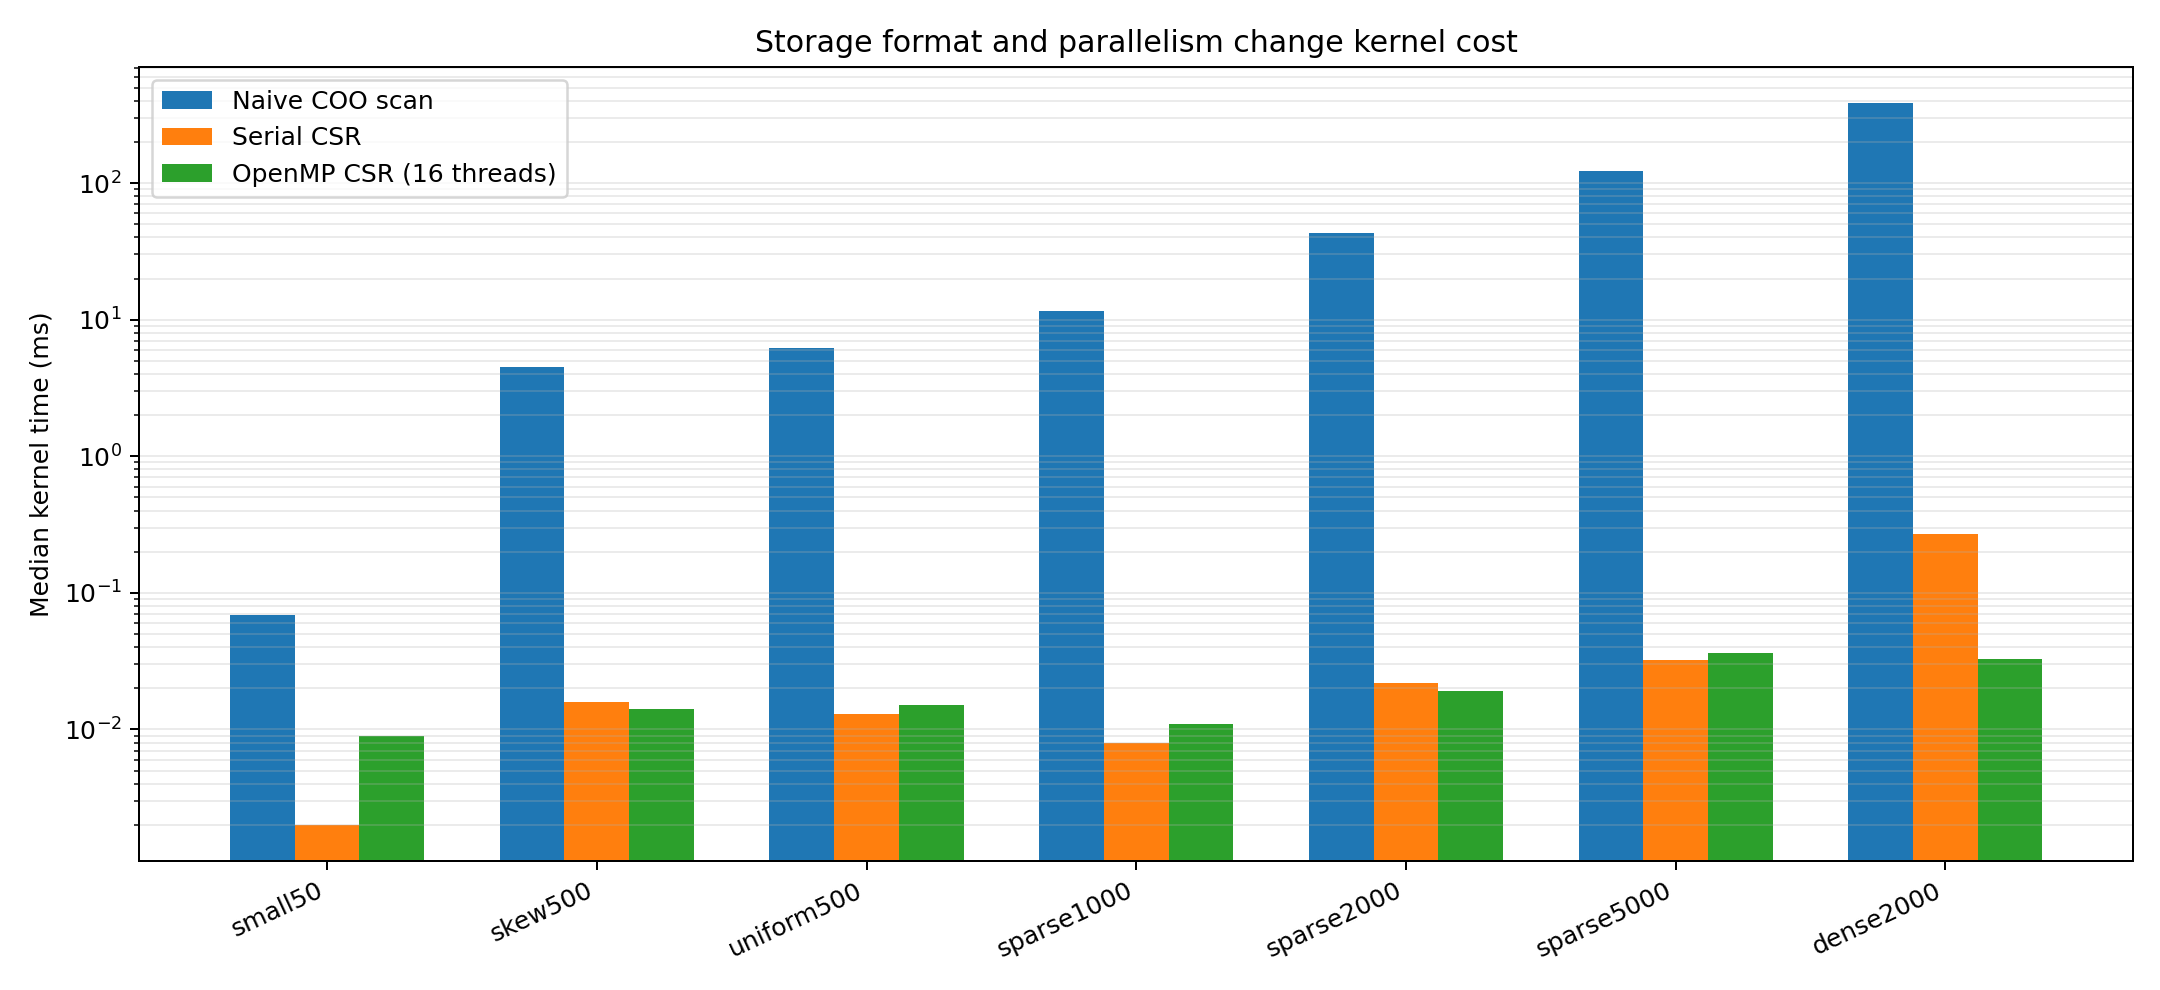
\includegraphics[width=0.9\linewidth]{figure/storage_runtime_comparison.png}
  \caption{Storage runtime comparison}
\end{figure}

\begin{figure}[h]
  \centering
  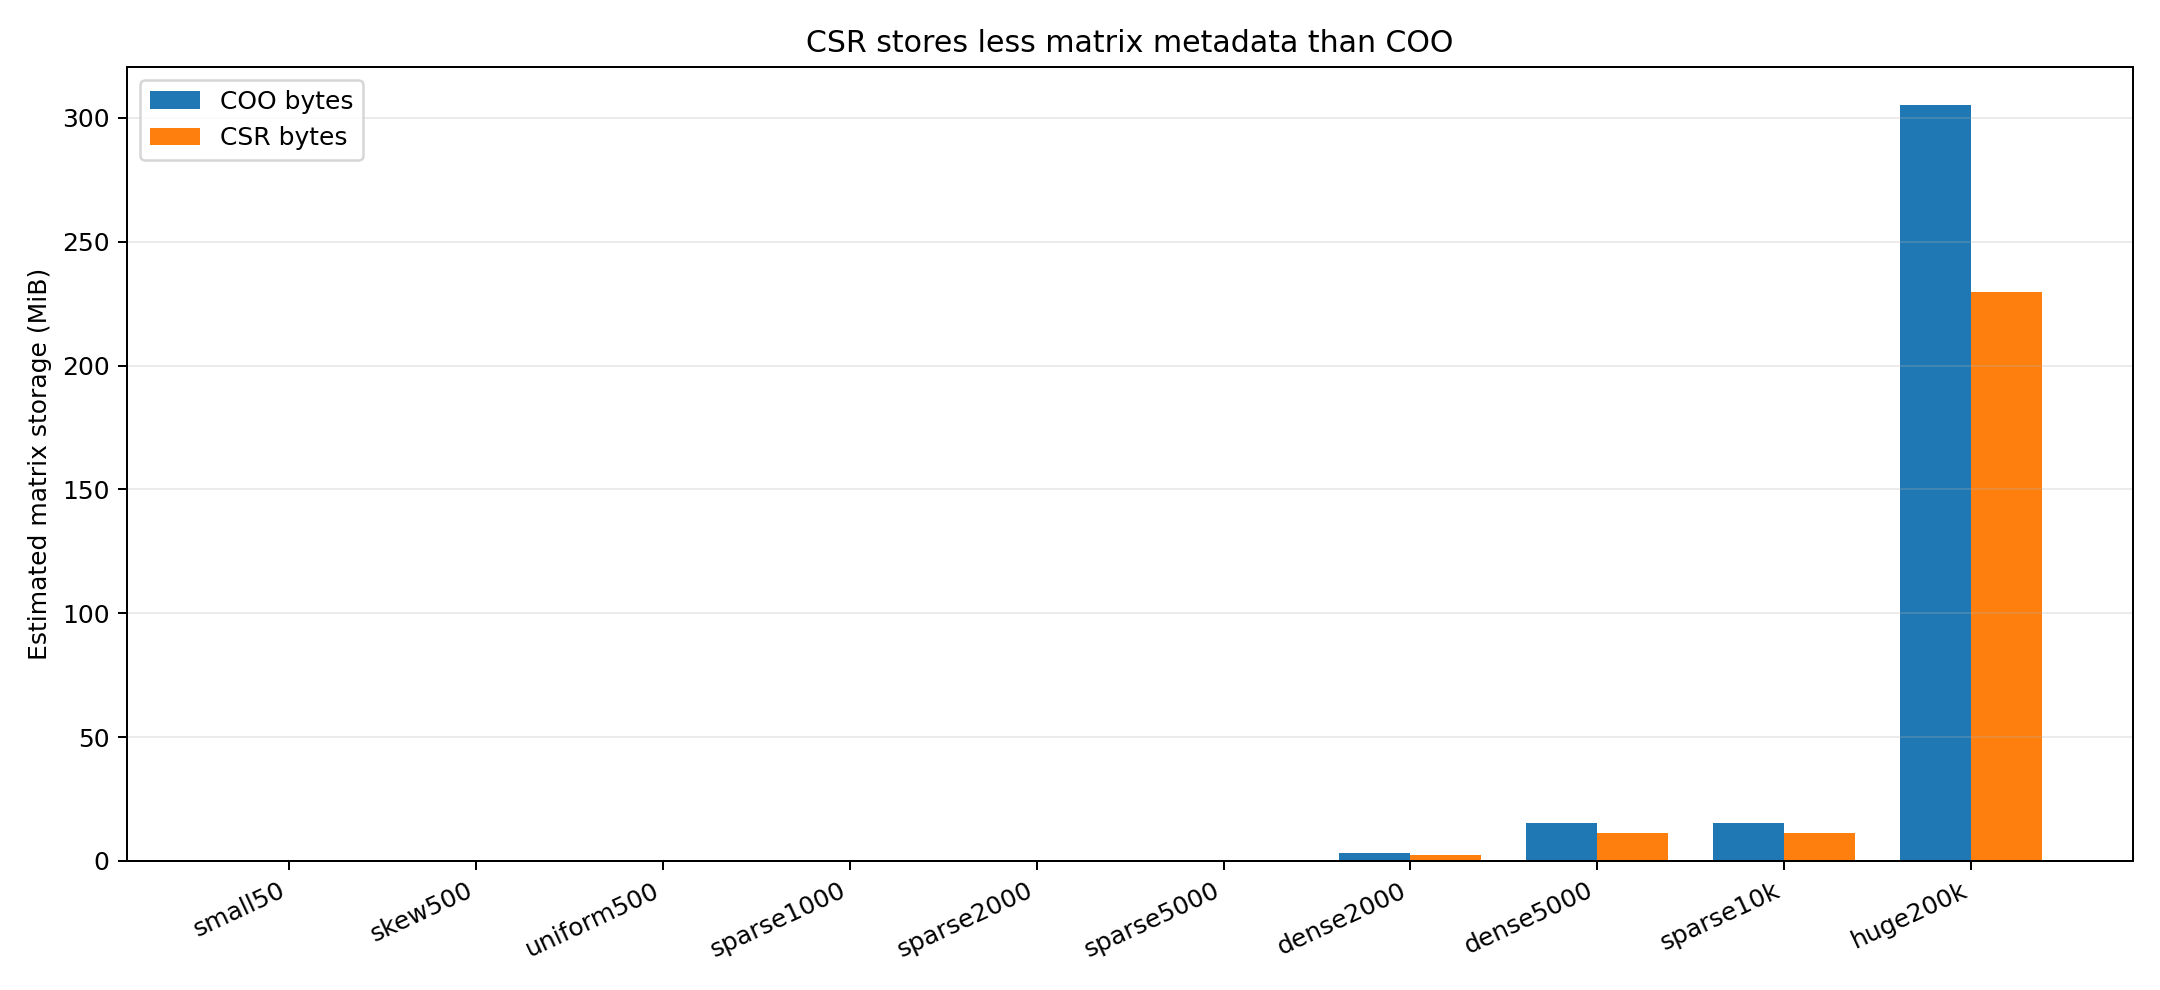
\includegraphics[width=0.9\linewidth]{figure/matrix_storage_footprint.png}
  \caption{Estimated matrix storage}
\end{figure}

\section{How Does Matrix Size Influence Performance?}

The dominant trend is that runtime scales with the amount of nonzero work, not just the row count. Figure 3 orders the matrices by \texttt{nnz}, and both CSR implementations follow that growth. Tiny matrices stay below 0.1 ms, the 1M-nnz matrices land around the sub-millisecond to low-millisecond range, and the 20M-nnz \texttt{huge\_200k\_100} case is the clear outlier.

On \texttt{large\_10000\_sparse\_100} (1,000,000 non-zeros), serial CSR needed 1.604 ms. On \texttt{huge\_200k\_100} (20,000,000 non-zeros), serial CSR rose to 38.41 ms. The 20x increase in non-zeros therefore produced roughly a 23.9x increase in kernel time, which is close to the work increase expected for SpMV.

\begin{figure}[h]
  \centering
  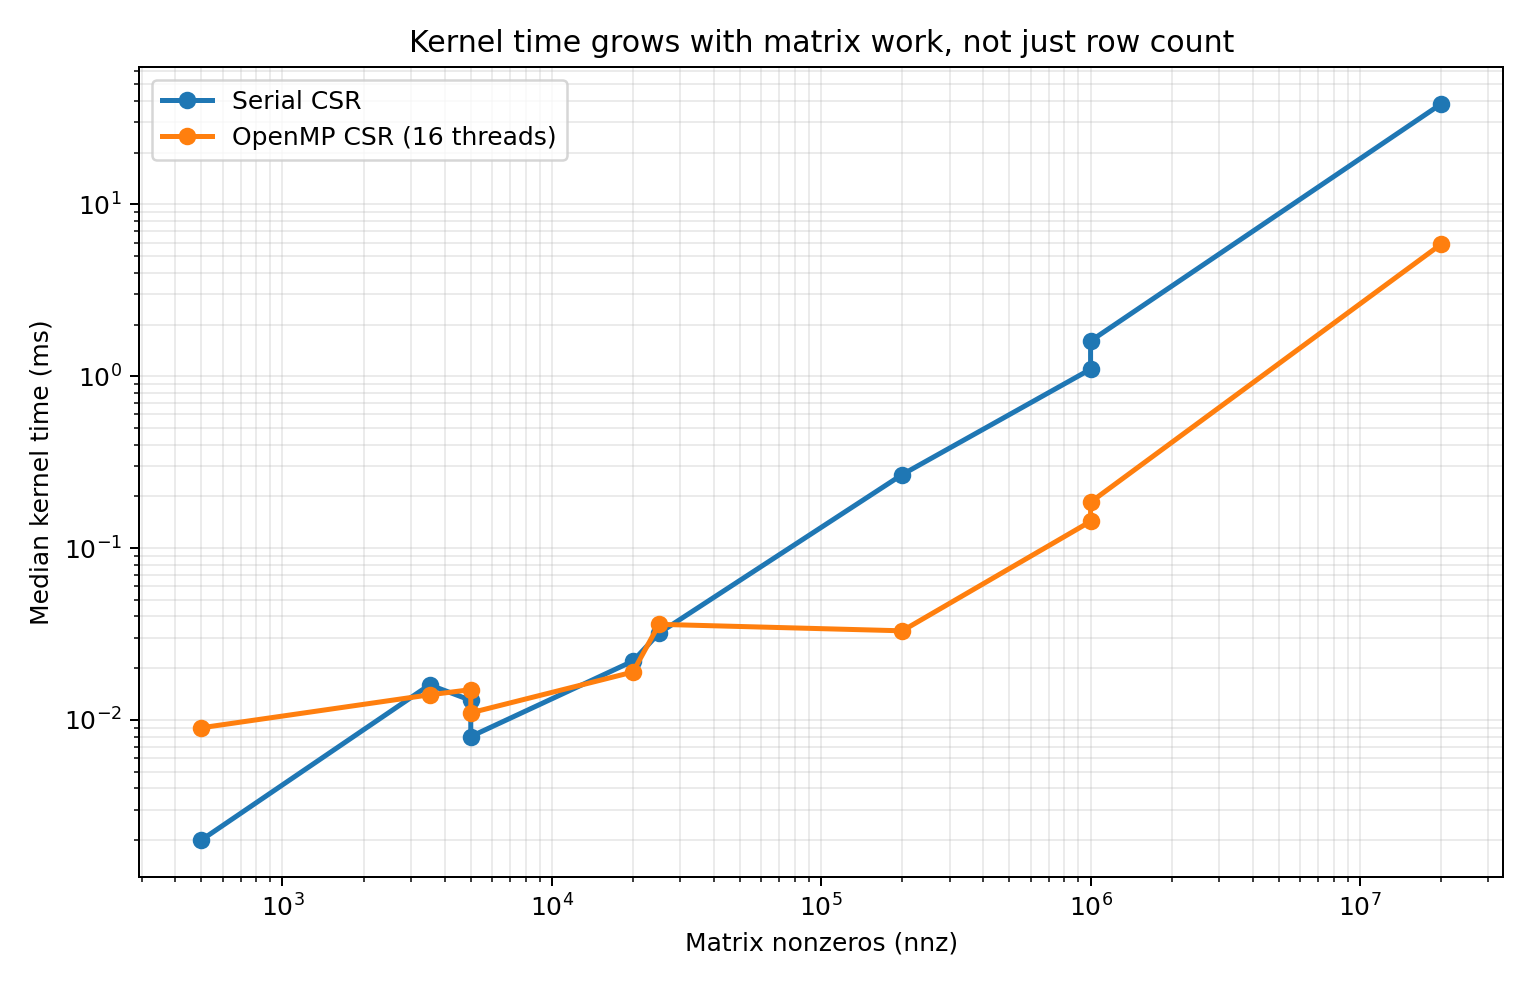
\includegraphics[width=0.9\linewidth]{figure/matrix_size_runtime.png}
  \caption{Matrix size vs runtime}
\end{figure}

\section{How Does the Number of Threads Influence Performance?}

The scaling behavior is strongly workload-dependent.

\begin{itemize}
  \item For \texttt{large\_sparse\_5000}, adding threads helps little after a point: 1-thread OpenMP took 0.0550 ms and 16 threads reached 0.0360 ms. The matrix is too small for thread startup, synchronization, and memory traffic to amortize perfectly.
  \item For \texttt{huge\_200k\_100}, the effect is much stronger: 1-thread OpenMP took 36.76 ms and 16 threads dropped to 5.864 ms.
\end{itemize}

In other words, more threads help when there is enough nonzero work and memory-level parallelism to keep the cores busy. On small matrices, parallel overhead dominates sooner.

\section{What Is the Speedup of the Parallel Code Compared to the Serial Version?}

The best 16-thread speedup in these experiments was on \texttt{large\_10000\_sparse\_100} at 8.67x over serial CSR. The weakest 16-thread speedup among the scaling datasets was on \texttt{large\_sparse\_5000} at 0.89x.

For the largest case, \texttt{huge\_200k\_100}, serial CSR took 38.41 ms and the 16-thread OpenMP kernel took 5.864 ms, which is a 6.55x speedup. On \texttt{large\_10000\_sparse\_100}, the 16-thread speedup was 8.67x.

Figure 4 plots both runtime and speedup versus thread count. The ideal line is included as a reference; the measured curves stay below it because SpMV is memory-bound and the rows do not all carry the same amount of work.

\begin{figure}[h]
  \centering
  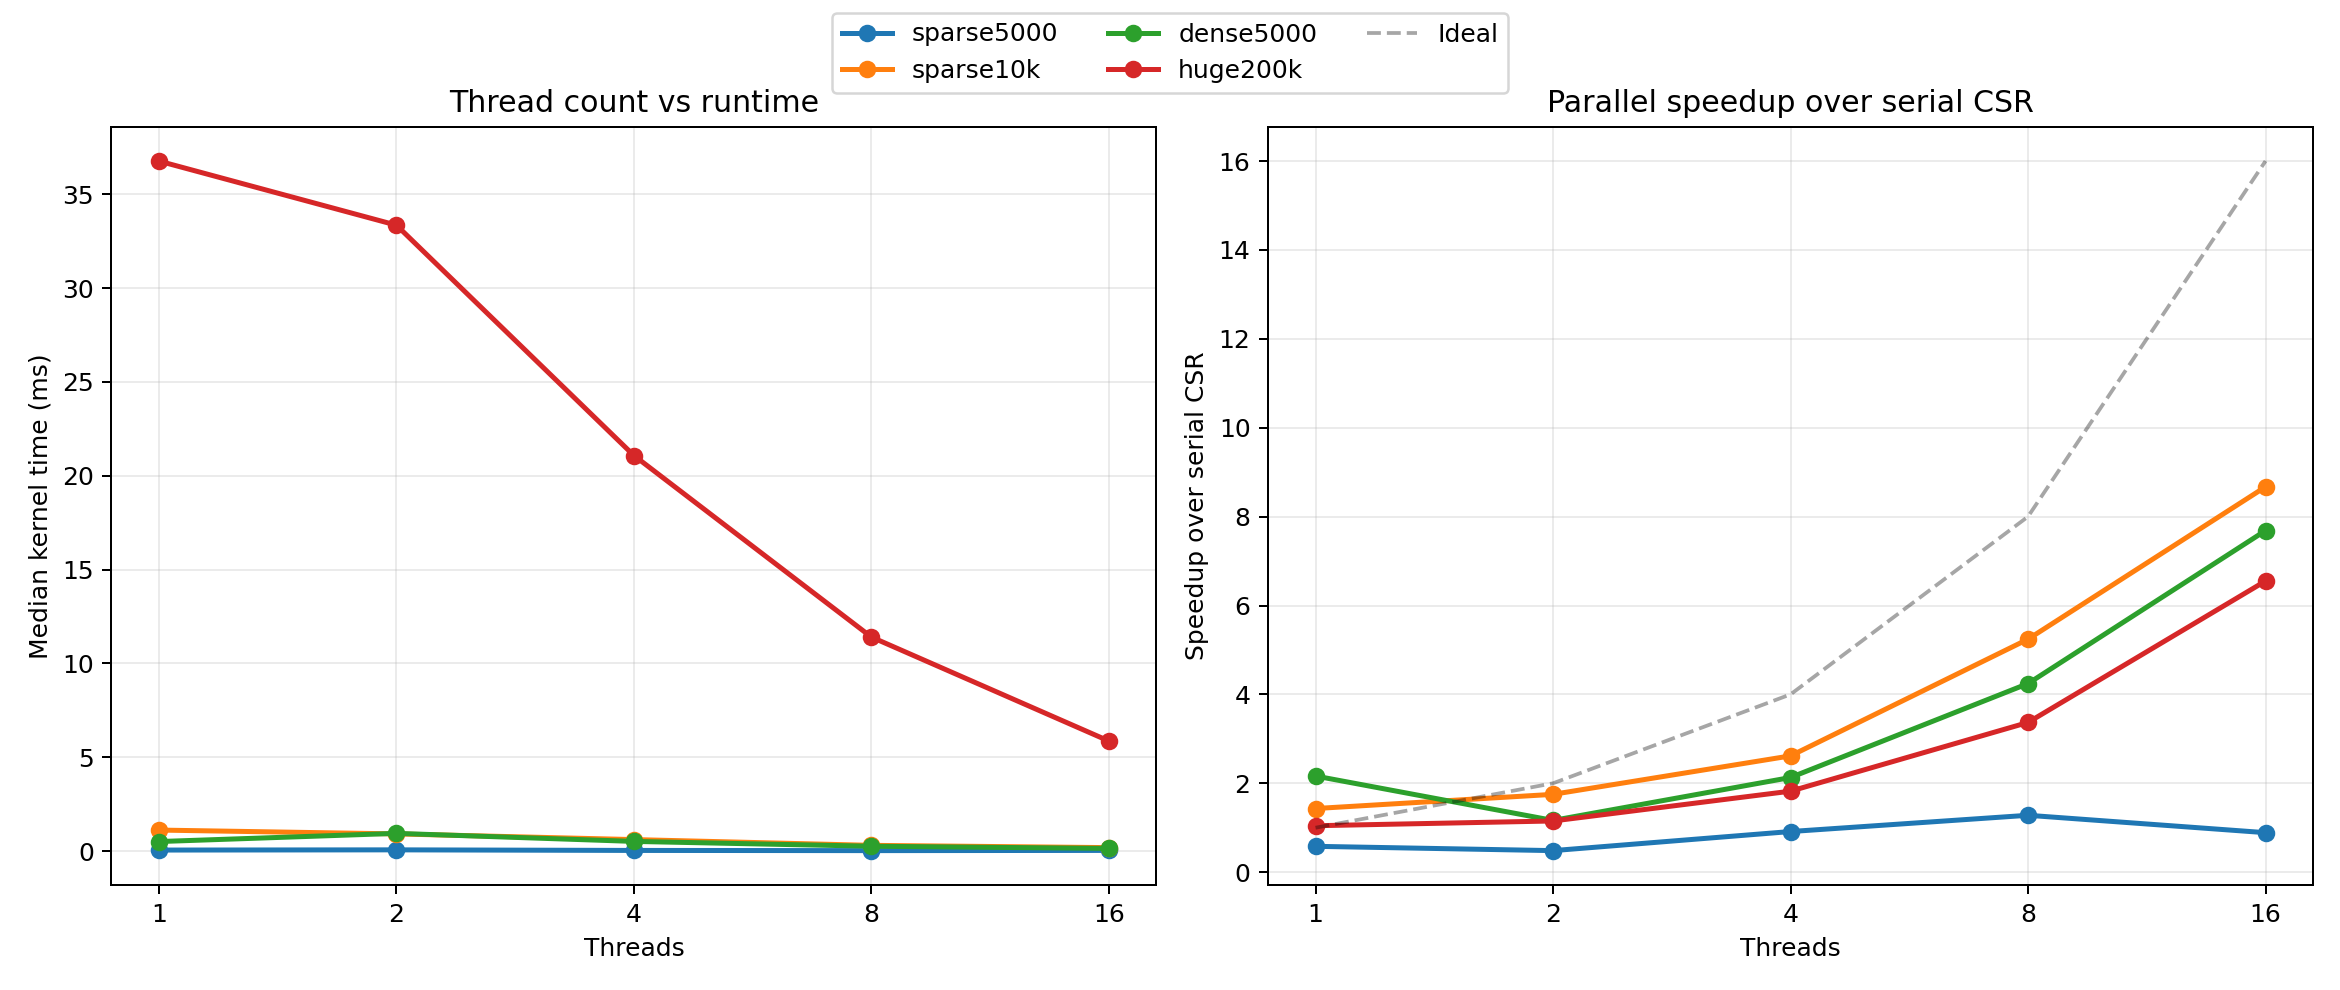
\includegraphics[width=0.9\linewidth]{figure/thread_scaling.png}
  \caption{Thread scaling and speedup}
\end{figure}

\section{Explain the Observed Scalability: Strong vs. Weak}

These experiments primarily measure strong scaling, not weak scaling. For each matrix, the problem size stays fixed while the thread count changes from 1 to 16. The plots therefore answer: how much faster does the same SpMV get when more threads are applied?

The results show moderate strong scaling on the larger matrices and weak strong scaling on the smaller ones. This is expected for SpMV because the kernel has low arithmetic intensity and quickly becomes limited by memory bandwidth, NUMA traffic, and synchronization overhead. The OpenMP implementation improves strong scaling by preserving locality: static row partitioning aligns with the first-touch initialization, thread pinning spreads threads across cores, and the optional thread-local copy of \texttt{x} reduces shared-vector contention for medium-size inputs.

A true weak-scaling study would increase matrix size proportionally with thread count so that each thread keeps roughly constant work. That was not the experiment required by the assignment questions here, so I describe the observed behaviour as strong scaling.

\section{Additional Insights}

\begin{itemize}
  \item Comparing \texttt{large\_sparse\_2000} and \texttt{large\_denserows\_2000} shows why nnz distribution matters. They have the same row count, but the denser matrix has 10x more non-zeros and correspondingly higher kernel time.
  \item The OpenMP version is not just ``serial CSR plus threads''. The NUMA-aware first-touch and thread pinning decisions match the dual-socket machine described in the spec, which is why the parallel code remains effective on the bigger matrices.
  \item The naive COO-scan baseline is useful for correctness and for demonstrating why CSR matters, but it stops being a practical performance baseline once matrices grow beyond the small and medium cases.
\end{itemize}

\section{Experiment Data Log}

\begin{itemize}
  \item Raw benchmark runs: \texttt{report\_raw\_results.csv}
  \item Summary metrics: \texttt{report\_metrics.json}
  \item Figure directory: \texttt{figure/}
\end{itemize}

\end{document}
